\section{Referencia de la Clase presupuesto}
\label{classpresupuesto}\index{presupuesto@{presupuesto}}
Administra la informaci\'{o}n de un presupuesto.  


{\tt \#include $<$presupuesto.h$>$}

Diagrama de herencias de presupuesto\begin{figure}[H]
\begin{center}
\leavevmode
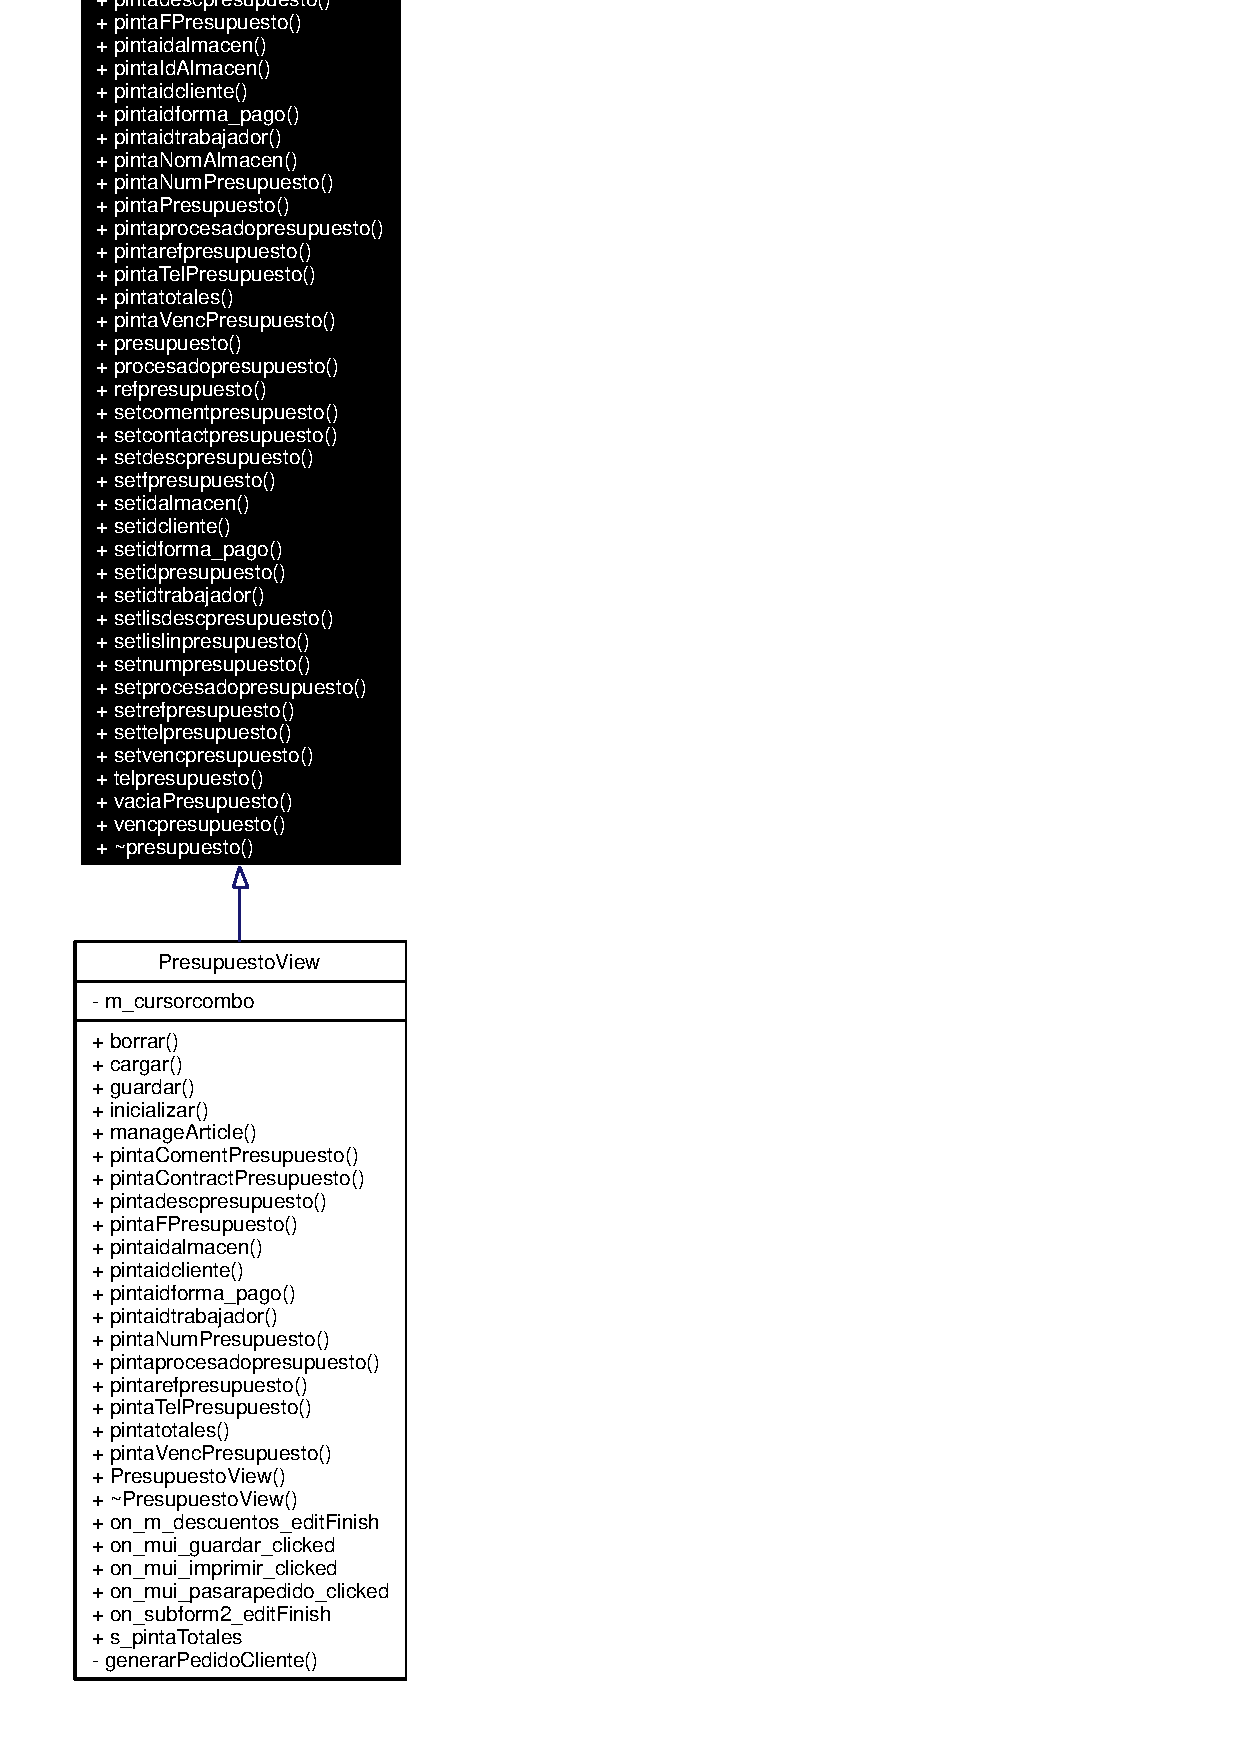
\includegraphics[width=97pt]{classpresupuesto__inherit__graph}
\end{center}
\end{figure}
Diagrama de colaboraci\'{o}n para presupuesto:\begin{figure}[H]
\begin{center}
\leavevmode
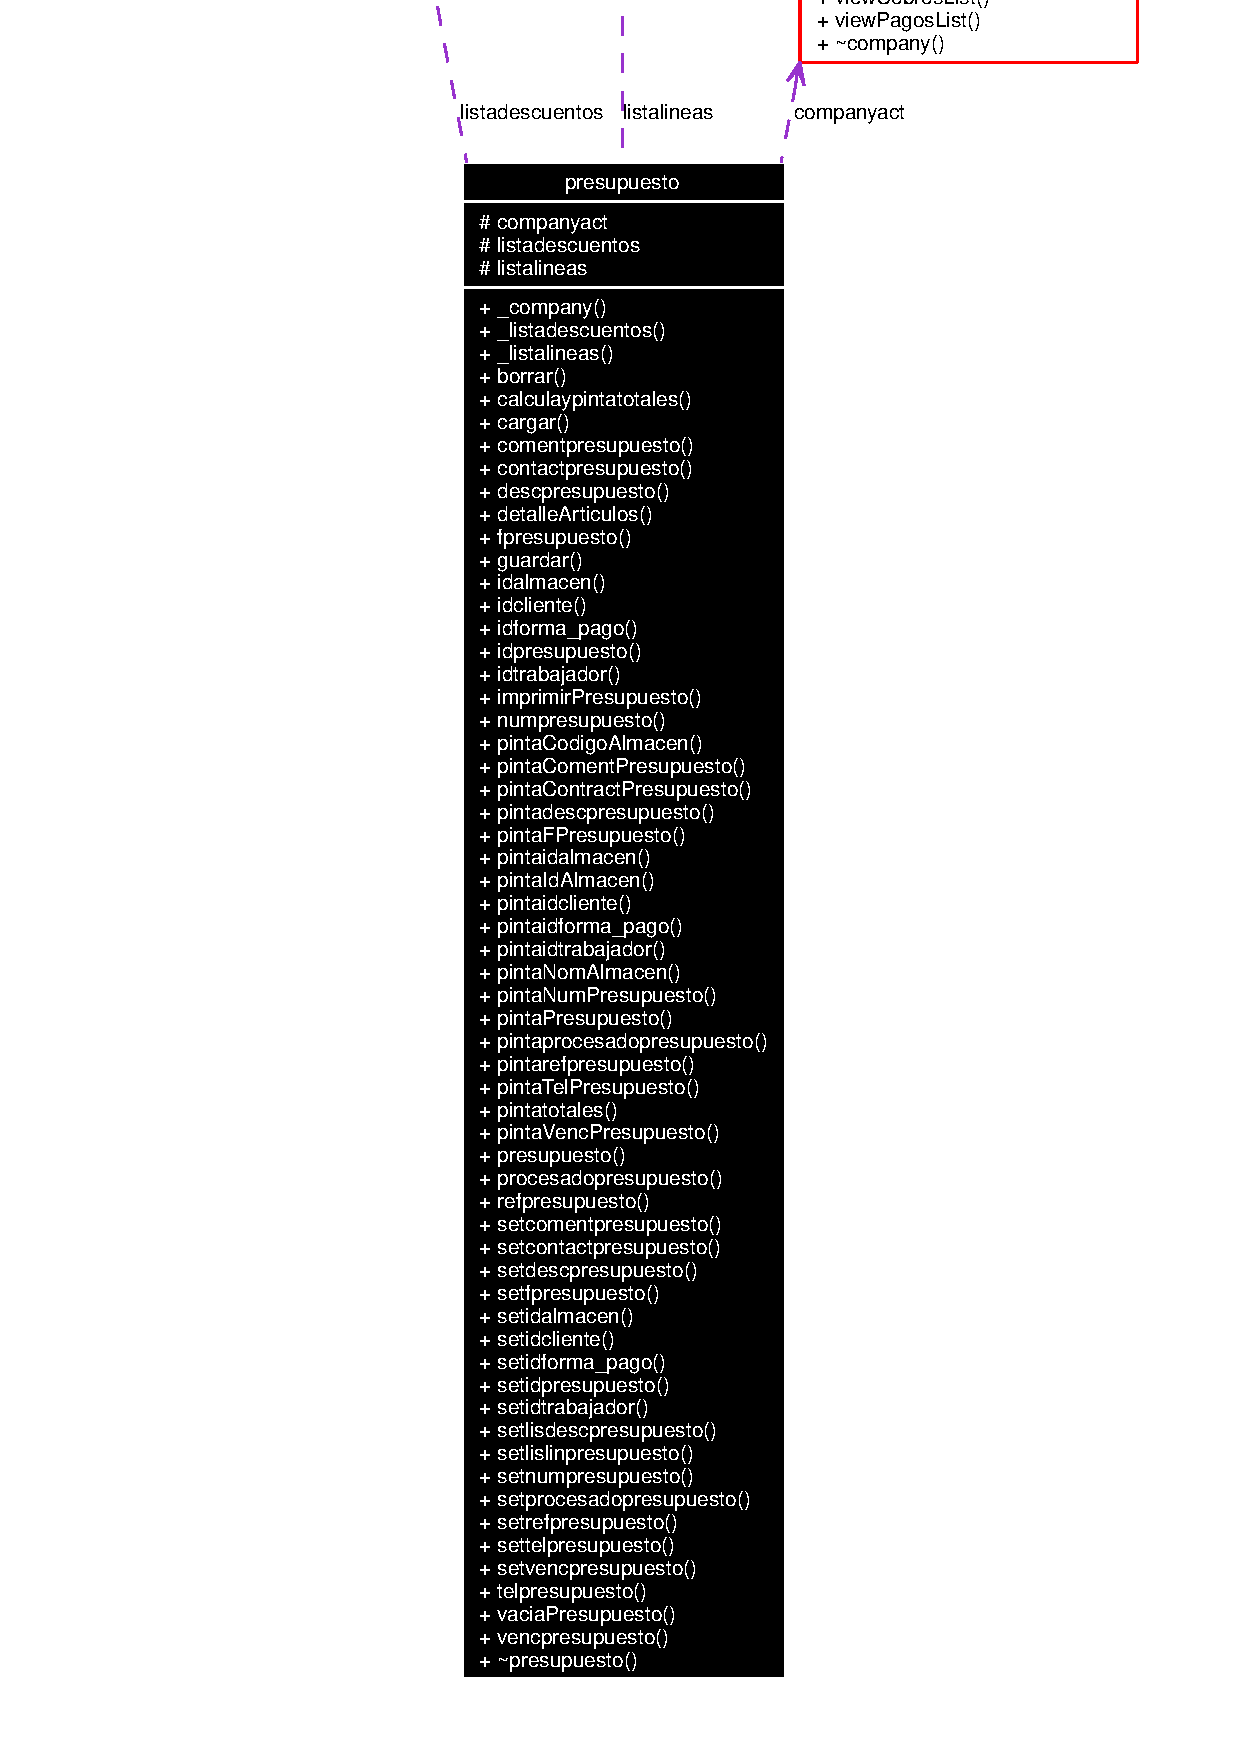
\includegraphics[width=273pt]{classpresupuesto__coll__graph}
\end{center}
\end{figure}
\subsection*{M\'{e}todos p\'{u}blicos}
\begin{CompactItemize}
\item 
{\bf company} $\ast$ {\bf \_\-company} ()\label{classpresupuesto_a0}

\item 
{\bf List\-Descuento\-Presupuesto\-View} $\ast$ {\bf \_\-listadescuentos} ()\label{classpresupuesto_a1}

\item 
{\bf listlinpresupuestoview} $\ast$ {\bf \_\-listalineas} ()\label{classpresupuesto_a2}

\item 
virtual int {\bf borrar} ()\label{classpresupuesto_a3}

\item 
virtual void {\bf calculaypintatotales} ()
\item 
virtual int {\bf cargar} (QString)
\begin{CompactList}\small\item\em Esta funcion carga un presupuesto. \item\end{CompactList}\item 
QString {\bf comentpresupuesto} ()\label{classpresupuesto_a6}

\item 
QString {\bf contactpresupuesto} ()\label{classpresupuesto_a7}

\item 
QString {\bf descpresupuesto} ()\label{classpresupuesto_a8}

\item 
virtual QString {\bf detalle\-Articulos} ()\label{classpresupuesto_a9}

\item 
QString {\bf fpresupuesto} ()\label{classpresupuesto_a10}

\item 
virtual int {\bf guardar} ()\label{classpresupuesto_a11}

\item 
QString {\bf idalmacen} ()\label{classpresupuesto_a12}

\item 
QString {\bf idcliente} ()\label{classpresupuesto_a13}

\item 
QString {\bf idforma\_\-pago} ()\label{classpresupuesto_a14}

\item 
QString {\bf idpresupuesto} ()\label{classpresupuesto_a15}

\item 
QString {\bf idtrabajador} ()\label{classpresupuesto_a16}

\item 
virtual void {\bf imprimir\-Presupuesto} ()
\item 
QString {\bf numpresupuesto} ()\label{classpresupuesto_a18}

\item 
virtual void {\bf pinta\-Codigo\-Almacen} (QString)\label{classpresupuesto_a19}

\item 
virtual void {\bf pinta\-Coment\-Presupuesto} (QString)\label{classpresupuesto_a20}

\item 
virtual void {\bf pinta\-Contract\-Presupuesto} (QString)\label{classpresupuesto_a21}

\item 
virtual void {\bf pintadescpresupuesto} (QString)\label{classpresupuesto_a22}

\item 
virtual void {\bf pinta\-FPresupuesto} (QString)\label{classpresupuesto_a23}

\item 
virtual void {\bf pintaidalmacen} (QString)\label{classpresupuesto_a24}

\item 
virtual void {\bf pinta\-Id\-Almacen} (QString)\label{classpresupuesto_a25}

\item 
virtual void {\bf pintaidcliente} (QString)\label{classpresupuesto_a26}

\item 
virtual void {\bf pintaidforma\_\-pago} (QString)\label{classpresupuesto_a27}

\item 
virtual void {\bf pintaidtrabajador} (QString)\label{classpresupuesto_a28}

\item 
virtual void {\bf pinta\-Nom\-Almacen} (QString)\label{classpresupuesto_a29}

\item 
virtual void {\bf pinta\-Num\-Presupuesto} (QString)\label{classpresupuesto_a30}

\item 
virtual void {\bf pinta\-Presupuesto} ()\label{classpresupuesto_a31}

\item 
virtual void {\bf pintaprocesadopresupuesto} (QString)\label{classpresupuesto_a32}

\item 
virtual void {\bf pintarefpresupuesto} (QString)\label{classpresupuesto_a33}

\item 
virtual void {\bf pinta\-Tel\-Presupuesto} (QString)\label{classpresupuesto_a34}

\item 
virtual void {\bf pintatotales} (Fixed, Fixed, Fixed, Fixed)\label{classpresupuesto_a35}

\item 
virtual void {\bf pinta\-Venc\-Presupuesto} (QString)\label{classpresupuesto_a36}

\item 
{\bf presupuesto} ({\bf company} $\ast$)\label{classpresupuesto_a37}

\item 
QString {\bf procesadopresupuesto} ()\label{classpresupuesto_a38}

\item 
QString {\bf refpresupuesto} ()\label{classpresupuesto_a39}

\item 
void {\bf setcomentpresupuesto} (QString val)\label{classpresupuesto_a40}

\item 
void {\bf setcontactpresupuesto} (QString val)\label{classpresupuesto_a41}

\item 
void {\bf setdescpresupuesto} (QString val)\label{classpresupuesto_a42}

\item 
void {\bf setfpresupuesto} (QString val)\label{classpresupuesto_a43}

\item 
void {\bf setidalmacen} (QString val)\label{classpresupuesto_a44}

\item 
void {\bf setidcliente} (QString val)\label{classpresupuesto_a45}

\item 
void {\bf setidforma\_\-pago} (QString val)\label{classpresupuesto_a46}

\item 
void {\bf setidpresupuesto} (QString val)\label{classpresupuesto_a47}

\item 
void {\bf setidtrabajador} (QString val)\label{classpresupuesto_a48}

\item 
void {\bf setlisdescpresupuesto} ({\bf List\-Descuento\-Presupuesto\-View} $\ast$a)\label{classpresupuesto_a49}

\item 
void {\bf setlislinpresupuesto} ({\bf listlinpresupuestoview} $\ast$a)\label{classpresupuesto_a50}

\item 
void {\bf setnumpresupuesto} (QString val)\label{classpresupuesto_a51}

\item 
void {\bf setprocesadopresupuesto} (QString val)\label{classpresupuesto_a52}

\item 
void {\bf setrefpresupuesto} (QString val)\label{classpresupuesto_a53}

\item 
void {\bf settelpresupuesto} (QString val)\label{classpresupuesto_a54}

\item 
void {\bf setvencpresupuesto} (QString val)\label{classpresupuesto_a55}

\item 
QString {\bf telpresupuesto} ()\label{classpresupuesto_a56}

\item 
void {\bf vacia\-Presupuesto} ()\label{classpresupuesto_a57}

\item 
QString {\bf vencpresupuesto} ()\label{classpresupuesto_a58}

\end{CompactItemize}
\subsection*{Atributos protegidos}
\begin{CompactItemize}
\item 
{\bf company} $\ast$ {\bf companyact}\label{classpresupuesto_p0}

\item 
{\bf List\-Descuento\-Presupuesto\-View} $\ast$ {\bf listadescuentos}\label{classpresupuesto_p1}

\item 
{\bf listlinpresupuestoview} $\ast$ {\bf listalineas}\label{classpresupuesto_p2}

\end{CompactItemize}


\subsection{Descripci\'{o}n detallada}
Administra la informaci\'{o}n de un presupuesto. 



\subsection{Documentaci\'{o}n de las funciones miembro}
\index{presupuesto@{presupuesto}!calculaypintatotales@{calculaypintatotales}}
\index{calculaypintatotales@{calculaypintatotales}!presupuesto@{presupuesto}}
\subsubsection{\setlength{\rightskip}{0pt plus 5cm}void presupuesto::calculaypintatotales ()\hspace{0.3cm}{\tt  [virtual]}}\label{classpresupuesto_a4}


Disparamos los plugins con presupuesto\_\-imprimir\-Presupuesto.

Impresion de los contenidos.

Impresion de los descuentos. \index{presupuesto@{presupuesto}!cargar@{cargar}}
\index{cargar@{cargar}!presupuesto@{presupuesto}}
\subsubsection{\setlength{\rightskip}{0pt plus 5cm}int presupuesto::cargar (QString {\em idbudget})\hspace{0.3cm}{\tt  [virtual]}}\label{classpresupuesto_a5}


Esta funcion carga un presupuesto. 

Tratamiento de excepciones. 

Reimplementado en {\bf Presupuesto\-View} {\rm (p.\,\pageref{classPresupuestoView_a1})}.\index{presupuesto@{presupuesto}!imprimirPresupuesto@{imprimirPresupuesto}}
\index{imprimirPresupuesto@{imprimirPresupuesto}!presupuesto@{presupuesto}}
\subsubsection{\setlength{\rightskip}{0pt plus 5cm}void presupuesto::imprimir\-Presupuesto ()\hspace{0.3cm}{\tt  [virtual]}}\label{classpresupuesto_a17}


Disparamos los plugins con presupuesto\_\-imprimir\-Presupuesto.

Copiamos el archivo.

Copiamos el logo

Linea de totales del presupuesto.

Impresion de la tabla de contenidos.

Contador que sirve para poner lineas de mas en caso de que sea preciso.

Impresion de los descuentos.

Impresion de los totales.

Rellena el primer tr de titulares.

Rellena el segundo tr de cantidades.

En la version para windows hay problemas con las imagenes, por eso de momento lo dejamos asi. 

La documentaci\'{o}n para esta clase fu\'{e} generada a partir de los siguientes archivos:\begin{CompactItemize}
\item 
presupuesto.h\item 
presupuesto.cpp\end{CompactItemize}
